\documentclass[../main.tex]{subfiles}
\begin{document}
\chapter{Analysis setup}
\label{hh:chapter:analysis}

This chapter describes the analysis strategy followed in the search for Higgs pair production via gluon-gluon fusion and vector boson fusion and decaying into two b quarks and two $\tau$ leptons. The aim of the analysis is to provide a value of the production cross section and study deviations from the Higgs boson couplings involved. However, since the statistics collected during the LHC Run 2 are not enough to provide this kind of results, an upper limit on the cross section of the HH produced via ggF and VBF will be obtained, and exclusion ranges on the couplings will be established. The statistical model considered and the results obtained are shown in Chapter~\ref{hh:chapter:results}.

Being the $\tau$ lepton an unstable particle, several final states can be reconstructed. As described in Section~\ref{intro:subsec:taus}, the $\tau$ lepton mainly decays into hadrons, with a total branching fraction of 64.8\%. Alternatively, it can decay leptonically into an electron, an electron neutrino and a $\tau$ neutrino or into a muon, a muon neutrino and a $\tau$ neutrino, with similar branching fractions of 17.8 and 17.4\%, respectively. These three decays are denoted as $\tau_h$, $\tau_e$, and $\tau_\mu$, respectively. The combination of $\tau$ decays leads to six possible decay combinations. However, only three will be considered in the analysis, the ones where at least one $\tau$ decays hadronically: the fully hadronic final state,\tauh\tauh{}, and the semi-leptonic ones, \taue\tauh{} and \taumu\tauh, covering 87.6\% of the total branching fraction. Additionally, at least two jets will also be present in the final state.

Signal extraction will be performed using simulated HH samples produced via ggF and VBF. In order to study possible BSM scenarios, several samples with different values of the Higgs boson couplings involved are produced, so they can be reweighted to generate distributions for other coupling values. The modelling of the signal processes and the reweighting methods are described in Section~\ref{hh:subsec:signal_modelling}.

Several processes have a final state that is the same or can mimic the final state of the HH~$\to$~bb$\tau\tau$ signal, contributing as background sources in the analysis. Two types of backgrounds are usually distinguished: irreducible backgrounds, whose final state is the same as in the signal, and reducible backgrounds, whose final state results as the one from the signal due to the misidentification of one or more objects. The modelling of these backgrounds is described in Section~\ref{hh:subsec:bkg_modelling}, although a minor description is given in the following.

Two processes constitute the major irreducible backgrounds. The first one is the production of pair of leptons through Drell-Yan (DY) processes (Z/$\gamma^*\to ll$) in association with jets. The two leptons can be associated to the decay products of one of the Higgs bosons and a pair of jets can be selected as the ones that come from the other Higgs decay. 

The other major irreducible background source in the pair production of top quarks (t$\bar{\text{t}}$). Each of the top quarks decays almost exclusively to a b quark and a W boson, which in turn can decay into a lepton and a neutrino or to a pair of quarks. This results in three possible t$\bar{\text{t}}$ decay final states: the di-leptonic final state, where the two W bosons decay into a lepton and a neutrino; the semi-leptonic final state, where one W boson decays leptonically and the other one into two quarks; and the fully-hadronic final-state, where both W bosons decay into quarks. The first two final states are the ones that give the highest contribution to the background, since the di-leptonic decay has the same final state as the signal and the semi-leptonic decay a similar final state (if one jet is misidentified as a lepton) but a higher branching ratio than the fully-leptonic decay.

The largest reducible background comes from QCD multijet events, where two jets are misidentified as leptons. This process has a relatively large contribution in the \tauh\tauh{} channel, but its contribution to the \taue\tauh{} and \taumu\tauh is smaller due to the stringent requirements set at analysis level to select prompt high $p_t$ isolated leptons from the signal process.

Finally, W+jets events, with one lepton coming from the W decay and one jet misidentified as a \tauh{}, have a minimal contribution thanks to the b jet requirements. There are other backgrounds whose contributions are even smaller, e.g. single Higgs boson events or di- and tri-vector boson production.

To increase the signal purity, several selections are applied to the objects that could belong to the signal final state. Section~\ref{hh:sec:objects} describes these selections. Section~\ref{hh:sec:analysis_flow} includes all the dedicated steps of the analysis: selecting the H$~\to\tau\tau$ and H$~\to~$bb candidates, the VBF jet selection, the event categorization and the signal extraction strategies. Finally, Section~\ref{hh:sec:background} describes the methods used to estimate and normalize the main backgrounds and Section~\ref{hh:sec:corrections} includes the corrections applied to the simulated events used in the analysis.




\section{Data and simulated samples}

This analysis uses the data collected at CMS at $\sqrt{s}=13$~TeV during 2016, 2017 and 2018, corresponding to integrated luminosities of 36.3, 41.5, and 59.7 fb${}^{-1}$ respectively. MC simulated samples, generated with programs based on state-of-the-art theoretical calculations, are used for both signal and background processes.

\subsection{Signal modelling}
\label{hh:subsec:signal_modelling}


The exploration of several BSM scenarios requires the modelling of the signals for several sets of couplings. As only a limited set of simulated samples can be produced, weighting techniques are implemented for both ggF and VBF HH signals, so additional BSM scenarios can be modelled starting only from a few BSM samples. 

Regarding ggF, the reweighting is based on the sum of different samples \cite{hh:analysis:ggf_reweighting}. At LO, the amplitude of the ggF production can be written as
\begin{equation}
\mathcal{A} = \kappa_\lambda\kappa_t T + \kappa_t^2 B,
\end{equation}
where $T$ and $B$ can be associated to the triangle and box diagrams of Fig.~\ref{hh:fig:ggf_feynman}. Therefore, the ggF production cross section can be computed from the square of the amplitude,
\begin{equation}
\label{hh:eq:ggf_sigma}
\sigma(\kappa_\lambda, \kappa_t) \sim |\mathcal{A}|^2 = \kappa_\lambda^2\kappa_t^2 t + \kappa_t^4b + \kappa_\lambda\kappa_t^3 i,
\end{equation}
where $t = |T|^2$, $b=|B|^2$ and $i=|TB^* + B^*T|$. Eq.~\eqref{hh:eq:ggf_sigma} can be rewritten in matricial form as
\begin{equation}
\label{hh:eq:ggf_sigma_vector}
\sigma(\kappa_\lambda, \kappa_t) = \mathbf{c}(\kappa_\lambda, \kappa_t) \cdot \mathbf{v},
\end{equation}
where $\mathbf{c}(\kappa_\lambda, \kappa_t) = (\kappa_\lambda^2\kappa_t^2, \kappa_t^4, \kappa_\lambda\kappa_t^3)$ is the vector of coupling constants and $\mathbf{v} = (t, b, i)$ is the vector of the values of the three components.

Given three particular samples with fixed values of $\kappa_\lambda$ and $\kappa_t$ and cross sections $\sigma_1$, $\sigma_2$ and $\sigma_3$, Eq.~\eqref{hh:eq:ggf_sigma_vector} can be expressed as a linear combination of these three samples:
\begin{equation}
\label{hh:eq:ggf_sigma_matrix_dev}
\left(
\begin{matrix}
\sigma_1 \\ \sigma_2 \\ \sigma_3
\end{matrix}
\right)
= 
\left(
\begin{matrix}
c_1^1 & c_1^2& c_1^3 \\
c_2^1 & c_2^2& c_2^3 \\
c_3^1 & c_3^2& c_3^3
\end{matrix}
\right)
\left(
\begin{matrix}
t \\ b \\ i
\end{matrix}
\right),
\end{equation}
where $(c_i^1, c_i^2, c_i^3)$ is the vector of coupling constants for each particular sample. In matricial form, Eq.~\eqref{hh:eq:ggf_sigma_matrix_dev} can be expressed as
\begin{equation}
\mathbf{\sigma} = \mathbf{C}\mathbf{v}.
\end{equation}

Inverting this equation and substituting the obtained expression of $\mathbf{v}$, Eq.~\eqref{hh:eq:ggf_sigma_vector} becomes
\begin{equation}
\label{hh:eq:ggf_sigma_final}
\sigma(\kappa_\lambda, \kappa_t) = \mathbf{c}(\kappa_\lambda, \kappa_t)~C^{-1}~\mathbf{\sigma}.
\end{equation}

Eq.~\eqref{hh:eq:ggf_sigma_final} shows that the ggF production cross section for generic values of $\kappa_\lambda$ and $\kappa_t$ can be obtained just as a linear combination of the cross sections of three given samples with fixed values of  $\kappa_\lambda$ and $\kappa_t$. Similarly, the distribution of a particular variable of a generic ggF samples can be obtained just by manipulating the same distribution in the three produced ggF samples.

To perform these studies, three ggF samples at NLO were produced using \textsc{powheg} with a fixed value of $\kappa_t=1$ and $\kappa_\lambda=1$, $\kappa_\lambda=2.45$ and $\kappa_\lambda=5$ (whose cross sections are shown in Table~\ref{hh:analysis:ggf_samples}). Additionally, another sample with $\kappa_\lambda=0$ was produced to test the performance of the reweighting method. Fig.~\ref{{hh:fig:ggf_rew_test}} shows a comparison between the HH system mass obtained directly from the sample with $\kappa_\lambda=0$ and the same distribution obtained by reweighting the histograms from the first three samples. The comparison results very satisfactorily, validating the reweighting method. 

\begin{table}[h!]
\begin{center}
\begin{tabular}{c | c}
$\kappa_\lambda$ & $\sigma$ (fb) \\ \hline
1    & 31.05 \\
2.45 & 13.12 \\
5    & 91.17
\end{tabular}
\caption{$\kappa_\lambda$ parameter values considered in the ggF HH$~\to~$bb$\tau\tau$ simulated samples used and their corresponding cross sections. $\kappa_t$ takes a value of 1 in all cases. Cross sections are taken from \cite{hh:analysis:xs}, although their values have to be scaled by $\sigma_{\text{NNLO+FTapprox}}/\sigma_\text{NLO}$.}
\label{hh:analysis:ggf_samples}
\end{center}
\end{table}

\begin{figure}[h!]
\begin{center}
\includegraphics[width=0.6\textwidth]{Images/ggf_kl0}
\end{center}
\caption{Distribution of the invariant mass of the HH system obtained (black) from a HH sample produced via gluon-gluon fusion with $\kappa_\lambda=0$ (red) by reweighting the $\kappa_\lambda=1$, $\kappa_\lambda=2.45$ and $\kappa_\lambda=5$ samples to produce the distribution expected from a $\kappa_\lambda=0$ sample.}
\label{hh:fig:ggf_rew_test}
\end{figure}

These NLO samples are used for both signal extraction and training the machine learning approach described in Section~\ref{hh:sec:multiclass}. To train the neural network used for signal extraction (described in Section~\ref{hh:subsec:signal_extraction}), additional LO samples with bigger statistics were generated using \textsc{MadGraph5\_aMC@NLO}.

A similar procedure as the one used for the ggF production mode is also used for VBF modelling. In this case, the HH production cross section can be written as
\begin{align}
\sigma(\kappa_V, \kappa_{2V}, \kappa_\lambda) &\sim |\kappa_V\kappa_\lambda A + \kappa_V^2 B + \kappa_{2V} C| ^2 \notag\\
&= \kappa_V^2\kappa_\lambda^2 a + \kappa_V^4 b + \kappa_{VV}^2 c + \kappa_V^3\kappa_\lambda i_{ab} + \kappa_V\kappa_{VV}\kappa_\lambda i_{ac} + \kappa_V^2\kappa_{VV} i_{bc},
\end{align}
where $A$, $B$ and $C$ can be associated to the diagrams from Fig.~\ref{hh:fig:vbf_feynman}, $a = |A|^2$, $b = |B|^2$, $c = |C|^2$ and $i_{ij}$ are the inference terms. Thus, the VBF signal can be modelled by summing six components $\mathbf{V}=(a, b, c, i_{ab}, i_{ac}, i_{bc})$, scaled by $\mathbf{K}=(\kappa_V^2\kappa_\lambda^2, \kappa_V^4, \kappa_{VV}^2, \kappa_V^3\kappa_\lambda, \kappa_V\kappa_{VV}\kappa_\lambda,  \kappa_V^2\kappa_{VV})$. By defining $\mathbf{M}$ as the $6\times6$ coefficient matrix and $\mathbf{\sigma}$ as the vector of the cross sections of six different samples, the cross section $\sigma_\text{target}$ of a generic sample with given $\kappa_V$, $\kappa_{2V}$ and $\kappa_\lambda$ can be obtained as
\begin{equation}
\sigma_\text{target} = \mathbf{K}\mathbf{M}^{-1}\mathbf{\sigma}.
\end{equation}

Similarly, the shape and yield of the distribution from a generic sample can be obtained by reweighting the same distribution obtained from six produced samples. The samples used in the analysis were generated at LO with \textsc{MadGraph5\_aMC@NLO} with the $\kappa_V$, $\kappa_{2V}$ and $\kappa_\lambda$ values shown in Table~\ref{hh:analysis:vbf_samples}. An additional LO sample with $\kappa_V=0.5$, $\kappa_{2V}=1$ and $\kappa_{\lambda}=1$ was also produced to perform closure tests on the reweighting method. Fig.~\ref{hh:fig:vbf_rew_test} shows a comparison between the HH system mass obtained directly from the sample with $\kappa_V=0.5$ and the same distribution obtained by reweighting the histograms from the six given samples. The comparison results very satisfactorily, validating the reweighting method. 



\begin{table}[h!]
\begin{center}
\begin{tabular}{c | c | c | c}
$\kappa_V$ & $\kappa_{2V}$ & $\kappa_\lambda$ & $\sigma$ (fb) \\ \hline
1   & 1 & 1 & 1.726 \\
1.5 & 1 & 1 & 66.018 \\
1   & 1 & 0 & 4.609 \\
1   & 1 & 2 & 1.423 \\
1   & 2 & 1 & 14.218 \\
1   & 0 & 1 & 27.08
\end{tabular}
\caption{Combinations of the ($\kappa_V$, $\kappa_{2V}, \kappa_\lambda$) parameter values considered in the VBF HH$~\to~$bb$\tau\tau$ simulated samples used and their corresponding cross sections.}
\label{hh:analysis:vbf_samples}
\end{center}
\end{table}





\begin{figure}[h!]
\begin{center}
\includegraphics[width=0.6\textwidth]{Images/vbf_0p5_1_1}
\end{center}
\caption{Distribution of the invariant mass of the HH system obtained (black) from a HH sample produced via vector boson fusion with $\kappa_{V}=0.5$ (and the other couplings set to their SM values) and (red) by reweighting the samples in Table~\ref{hh:analysis:vbf_samples} to produce the distribution expected for a sample with $\kappa_{V}=0.5$.}
\label{hh:fig:vbf_rew_test}
\end{figure}

\subsection{Background modelling}
\label{hh:subsec:bkg_modelling}

Simulated events are generally used to predict the background contributions in this analysis.

Z/$\gamma^*\to ll$~+~jets is modelled with \textsc{MadGraph5\_aMC@NLO} at LO accuracy and normalized to its cross section computed at NNLO. The agreement between data and the simulation is improved by applying weights derived from dedicated Z$~\to~\mu\mu$ control regions, as shown in Section~\ref{hh:subsec:dy}. 

t$\bar{\text{t}}$ production is modelled with \textsc{POWHEG} at NLO, and its cross section is extracted by fitting in a t$\bar{\text{t}}$ control region (see Section~\ref{hh:subsec:tt}).

QCD multi-jet background is estimated fully from data, as shown in Section~\ref{hh:subsec:qcd}.

All background processes considered, their modelling approaches and the cross sections used are summarized in Table~\ref{hh:analysis:samples}.


\begin{table}[p]
\begin{footnotesize}
\begin{center}

%\begin{adjustbox}{width=\textwidth}
	\begin{tabular}{l | l | l}
		\hline\hline
		Process & Modelling (accuracy) & $\sigma\times\mathrm{B}$ (pb) \\\hline\hline
		Z/$\gamma^*\to ll~+~$Jets & \textsc{MadGraph5\_aMC@NLO} (LO) & 6077.22 \\\hline
		$\text{t}\bar{\text{t}}$ & \textsc{Powheg} (NLO) & \\
		\quad $\to~$Di-leptonic & & 88.29 \\
		\quad $\to~$Semi-leptonic & & 365.34 \\
		\quad $\to~$Fully-hadronic & & 377.96 \\
\hline
	 	QCD multijet & Data-driven (Section~\ref{hh:subsec:qcd}) & \\
\hline
		W$~\to l\nu~+~$Jets &  \textsc{MadGraph5\_aMC@NLO} (LO) & 61526.7\\
\hline
		Electroweak & \textsc{MadGraph5\_aMC@NLO} (LO) & \\
		W${}^+~+~$jj & & 25.62 \\
		W${}^-~+~$jj & & 20.25 \\
		Z + jj & & 3.987 \\
\hline
		Single-t (Single-$\bar{\text{t}}$) & \textsc{Powheg} (NLO) & \\
		W-channel & & 35.85 (35.85) \\
		t-channel & & 136.02 (80.95) \\
\hline
		WW & \textsc{Powheg} (NLO) & \\
		\quad$~\to 2l2\nu$ & & 12.18 \\
		\quad$~\to 2l2q$ & & 50.0 \\
		\quad$~\to 4q$ & & 51.72 \\
\hline
		ZZ & \textsc{Powheg} (NLO) & \\
		\quad$~\to 4l$ & & 1.26 \\
		\quad$~\to 2l2\nu$ & & 0.564 \\
		\quad$~\to 2l2q$ & & 5.52 \\
		\quad$~\to 2q2\nu$ & & 4.07 \\
\hline
		WZ & & \\
		\quad$~\to 3l\nu$ & \textsc{Powheg} (NLO) & 4.43 \\
		\quad$~\to l\nu2q$ & \textsc{MadGraph5\_aMC@NLO} (NLO) & 10.71 \\
		\quad$~\to l3\nu$ & \textsc{MadGraph5\_aMC@NLO} (NLO) & 3.06 \\
		\quad$~\to 2l2q$ & \textsc{MadGraph5\_aMC@NLO} (NLO) & 10.71 \\
\hline
		Triboson & \textsc{MadGraph5\_aMC@NLO} (NLO) & \\
		WWW &  & 0.209 \\
		WWZ &  & 0.168 \\
		WZZ &  & 0.057 \\
		ZZZ &  & 0.0147 \\
\hline
		Single Higgs & \textsc{Powheg} (NLO) & \\
		ggH (H$~\to\tau\tau$) & & 3.07 \\
		VBFH  (H$~\to\tau\tau$) & & 0.238 \\
		ttH & & \\
		\quad H$~\to~$bb & & 0.29 \\
		\quad H$~\to\tau\tau$ (2017-18) & & 0.032 \\
		\quad H$~\not\to~$bb & & 0.214 (2016), 0.182 (2017-18) \\
		WH (H$~\to\tau\tau$) & & 0.0858 \\
		ZH (H$~\to~$bb) & & \\
		\quad Z$~\to ll$ & & 0.05 \\
		\quad Z$~\to qq$ & & 0.35 \\
		ZH (H$~\to\tau\tau$) & & 0.0556\\
\hline
		$\text{t}\bar{\text{t}}$W (W$~\to l\nu$, $qq$) & \textsc{MadGraph5\_aMC@NLO} (NLO) & 0.61 \\
		$\text{t}\bar{\text{t}}$Z (Z$~\to 2l2\nu$) & \textsc{MadGraph5\_aMC@NLO} (NLO) & 0.2529 \\
		$\text{t}\bar{\text{t}}$WW & \textsc{MadGraph5\_aMC@NLO} (LO) & 0.000698 \\
		$\text{t}\bar{\text{t}}$WZ & \textsc{MadGraph5\_aMC@NLO} (LO) & 0.000244 \\
		$\text{t}\bar{\text{t}}$ZZ & \textsc{MadGraph5\_aMC@NLO} (LO) & 0.000139 \\
	\end{tabular}
%\end{adjustbox}
\end{center}
\end{footnotesize}
\caption{Background processes, models used and cross sections.}
\label{hh:analysis:samples}
\end{table}




\section{Physics objects preselection}
\label{hh:sec:objects}

A first selection on the reconstructed objects is performed to increase the signal purity. As the final state of the signal processes is two opposite-sign b quarks and the decay products of the $\tau\tau$ pair (electron and $\tau_h$, muon and $\tau_h$ or two $\tau_h$) and two additional forward jets in the case of VBF production, this selection targets jets, muons, electrons and $\tau_h$.


\textcolor{red}{How to choose the primary vertex will be explained in the PF section}

\subsection{Muons}
\label{hh:subsec:muons}

Muons in the analysis are reconstructed as explained in Section~{intro:subsec:muon} and are only selected if they pass the tight identification working point and the tight isolation working point (correspondent to $I^\mu_{rel}<0.15$). To ensure the compatibility of the muon candidate with the primary vertex, the distance between the muon track and the primary vertex must be in the transverse plane $d_{xy}<0.045$~cm  and in the longitudinal plane $d_z<0.2$~cm.

\subsection{Electrons}
\label{hh:subsec:electrons}

Electron identification is performed using the MVA described in Section~{intro:subsec:ele}. The tight working point, characterized by an 80$\%$ efficiency, is used in the analysis. The same $d_{xy}<0.045$~cm and $d_z<0.2$~cm requirements as for muons are imposed.

\subsection{Hadronic taus}
\label{hh:subsec:taus}

Decays of $\tau$ leptons into hadrons and a neutrino are reconstructed by the HPS identification algorithm, as described in Section~\ref{intro:subsec:taus}. In the analysis only the decays into h${}^\pm$,  h${}^\pm \pi^0$, h${}^\pm\pi^0\pi^0$, and h${}^\pm$h${}^\mp$h${}^\pm$ are considered. In order to discriminate the correct hadronic $\tau$ decays from quark and gluon jets and from electrons and muons, the three \deeptau{} discriminants will be considered. Different working points (as described in Section~\ref{intro:subsec:taus}) will be used depending on the $\tau$ pair decay channel. $\tau_h$ candidates are also asked to fulfil the $d_z<0.2$~cm requirement.


\subsection{Jets}
\label{hh:subsec:jets}

Both AK4 and AK8 jets, described in Section~\ref{intro:subsec:jets} are considered. b and VBF jet candidates are reconstructed as AK4 jets with $p_T>20$~GeV ($p_T>30$~GeV for VBF jets). VBF jets are reconstructed within $\eta<|4.7|$. Since b-tagging relies on the information from the tracker and this is only available in the central region, b jet candidates are required to be with $|\eta|<2.4$. In 2017, all jets with $20<p_T<50$ and $2.65<|\eta|<3.139$ are removed since they populate a very specific phase space region where is known 2017 MC simulation does not match the data.

All jets are required to pass the tight working point of the particle-flow jet identification. Jets with $p_T<50$~GeV are also required to pass the loose pile-up jet ID discriminator working point.

Depending on the separation $\Delta R_{jj}$ between the two b jets finally identified s coming from the Higgs decay, there are three possible regimes. If $\Delta R_{jj} > 0.8$, they will be reconstructed as two different AK4 jets. If $0.4 < \Delta R_{jj} < 0.8$, the jets are partially in overlap and they will be reconstructed as two different AK4 and jets and also as one merged AK8 jet. Finally, if $\Delta R_{jj} < 0.4$, the two jets will be reconstructed as one merged AK8 jet. The two final regimes correspond to the boosted production. However, for non resonant HH production, the latest highly boosted regime won't be reached. Therefore, events will be classified into two categories, the \textit{resolved} and the \textit{boosted} categories, associated to the $\Delta R_{jj} > 0.8$ and $0.4 < \Delta R_{jj} < 0.8$ topologies, respectively.



\section{Analysis flow}
\label{hh:sec:analysis_flow}

\subsection{$\text{H}\to\tau\tau$ pair selection}
\label{hh:subsec:htt_pair_selection}

As initial step, the decay products of the H$~\to\tau\tau$ decay are identified, considering the three decay modes described ($\tau_\mu\tau_h$, $\tau_e\tau_h$ and $\tau_h\tau_h$). 

After applying the preselection described in Section~\ref{hh:sec:objects} on the muons, electrons and hadronic $\tau$, the $\tau\tau$ decay mode is assessed. All signal events are required to have at least one hadronic $\tau$. Events are classified as \taumu\tauh{} if a muon satisfying the baseline selection is found, otherwise are classified as \taue\tauh{} if a baseline-electron is found and lastly as \tauh\tauh{} if two hadronic $\tau$ are present. For each channel, if more than one pair is found, they are sorted according to the isolation of the muon or the electron in the \taumu\tauh{} and \taue\tauh{} channels and the highest isolated $\tau_h$ (i.e. the one with the highest DeepTauVSjet score) in the \tauh\tauh{} channel.

Additionally to the preselection described in Sections \ref{hh:subsec:muons}, \ref{hh:subsec:electrons}, and \ref{hh:subsec:taus}, a kinematic selection is applied to the different objects depending on the trigger strategy followed, which depends on the channel considered. A summary of these triggers and the $p_t$ thresholds applied to the trigger objects is included in Table~\ref{hh:tab:triggers}. In the semileptonic channels, single-lepton and cross-lepton triggers are used. The single-lepton triggers require an isolated muon or electron, while the cross-triggers require an additional hadronic $\tau$. The cross-lepton triggers allow to reduce the threshold on the lepton $p_T$, increasing the acceptance of the analysis. Online $p_t$ thresholds vary between triggers and years. In 2016, the single-$\mu$ trigger required a muon of 22~GeV, while the cross trigger $\mu\tau_h$ required a muon of 19~GeV and a $\tau_h$ of 20~GeV. These numbers increased in 2017 and 2018 to 24~GeV for the single-$\mu$ trigger and 20 and 27~GeV for the cross trigger. Similarly, during the 2016 (2017-2018) campaign single-e triggers required a 25 (32)~GeV electron, while cross triggers $e\tau_h$ (only available in 2017 and 2018) required a 24~GeV electron and a 30~GeV $\tau_h$. For the \tauh\tauh{} channel, a double-\tauh{} trigger was used during the three years, requiring two 35~GeV \tauh{}. Additionally, during 2017 a new double-$\tau_h$ trigger targeting VBF production was introduced to increase the \tauh\tauh{} channel phase-space, so on top of requiring two 20~GeV \tauh{}, one jet with $p_T>115$~GeV and another one with $p_T>45$~GeV are needed at trigger level. All electrons, muons, and hadronic $\tau_h$ selected are required to be within $|\eta| < 2.1$.

\begin{table}[h!]
\begin{center}
\begin{tabular}{c | c | c}
$\tau\tau$ channel & Year & Trigger $p_T$ thresholds \\\hline\hline
\multirow{5}{*}{\taumu\tauh{}} 
  & 2016 & 
    \begin{tabular}{c}
      Single-$\mu$: $p_t^\mu > 22$~GeV \\
      Cross $\mu\tau_h$: $p_t^\mu > 20$~GeV, $p_t^{\tau_h} > 20$~GeV

	\end{tabular}\\\cline{2-3}
  & 2017 & 
    \begin{tabular}{c}
      Single-$\mu$: $p_t^\mu > 24$~GeV \\
      Cross $\mu\tau_h$: $p_t^\mu > 20$~GeV, $p_t^{\tau_h} > 27$~GeV

	\end{tabular}\\\cline{2-3}
  & 2018 & 
    \begin{tabular}{c}
      Single-$\mu$: $p_t^\mu > 24$~GeV \\
      Cross $\mu\tau_h$: $p_t^\mu > 20$~GeV, $p_t^{\tau_h} > 27$~GeV

	\end{tabular}\\\hline

\multirow{5}{*}{\taue\tauh{}} 
  & 2016 & 
    \begin{tabular}{c}
      Single-$e$: $p_t^e > 25$~GeV \\
	\end{tabular}\\\cline{2-3}
  & 2017 & 
    \begin{tabular}{c}
      Single-$e$: $p_t^e > 32$~GeV \\
      Cross $e\tau_h$: $p_t^e > 24$~GeV, $p_t^{\tau_h} > 30$~GeV

	\end{tabular}\\\cline{2-3}
  & 2018 & 
    \begin{tabular}{c}
      Single-$e$: $p_t^e > 32$~GeV \\
      Cross $e\tau_h$: $p_t^e > 24$~GeV, $p_t^{\tau_h} > 30$~GeV
	\end{tabular}\\\hline

\multirow{5}{*}{\tauh\tauh{}} 
  & 2016 & 
    \begin{tabular}{c}
      Double-$\tau_h$: $p_t^{\tau_h} > 35$~GeV \\
	\end{tabular}\\\cline{2-3}
  & 2017 & 
    \begin{tabular}{c}
      Double-$\tau_h$: $p_t^{\tau_h}> 35$~GeV \\
      VBF+H$~\to$~\tauh\tauh{} trigger: $p_t^{\tau_h} > 20$~GeV

	\end{tabular}\\\cline{2-3}
  & 2018 & 
    \begin{tabular}{c}
      Double-$\tau_h$: $p_t^{\tau_h} > 35$~GeV \\
      VBF+H$~\to$~\tauh\tauh{} trigger: $p_t^{\tau_h} > 20$~GeV
	\end{tabular}\\

\end{tabular}
\end{center}
\caption{Trigger selections applied in the analysis splitted by channel and year.}
\label{hh:tab:triggers}
\end{table}

Each reconstructed offline object is required to geometrically match (within $\Delta R < 0.5$) their corresponding trigger object and also pass a $p_T$ threshold depending on the HLT trigger fired by the event,
\begin{equation}
p_t^{\text{offline}} >= p_t^{\text{trigger}} + \text{offset},
\end{equation}
where $p_t^{\text{offline}}$ and $p_t^{\text{trigger}}$ are the $p_t$ of the offline object and the $p_t$ threshold of the trigger object respectively and $\text{offset}$ is a quantity chosen to be conservative with respect to the trigger turn-on curves. This offset depends on the lepton type: 1~GeV for electrons and muons and 5~GeV for hadronic $\tau$. Events passing the single-lepton triggers also require an hadronic \tauh{} of 20~GeV and $|\eta| < 2.3$. 

All selections applied to offline objects are summarized in Tables \ref{hh:tab:sel_mutau}, \ref{hh:tab:sel_etau} and \ref{hh:tab:sel_tautau}. Additional selections are applied to the lepton pair to increase the signal purity, such as both $\tau$ candidates having opposite charge or a spatial separation between them of $\Delta R > 0.5$.



\begin{table}[h!]
\begin{center}
\begin{tabular}{c|c|c}
	Object & Year & Selections \\\hline\hline
    \multirow{8}{*}{$\mu$}
    	&\multirow{1}{*}{All}  &
    		\begin{tabular}{c}
				Tight ID, Tight Iso. \\
				$|\eta|<2.1$ \\
				$d_{xy} < 0.045$~cm, $d_z < 0.2$~cm 
    		\end{tabular}\\\cline{2-3}
	    &\multirow{1}{*}{2016}  &
	    	\begin{tabular}{c}
				single-$\mu$: $p_t > 23$~GeV \\
				cross $\mu$\tauh{}: $p_t > 20$~GeV
    		\end{tabular}\\\cline{2-3}
	    &\multirow{1}{*}{2017}  &
	    	\begin{tabular}{c}
				single-$\mu$: $p_t > 25$~GeV \\
				cross $\mu$\tauh{}: $p_t > 21$~GeV
    		\end{tabular}\\\cline{2-3}
    	&\multirow{1}{*}{2018}  &
	    	\begin{tabular}{c}
				single-$\mu$: $p_t > 25$~GeV \\
				cross $\mu$\tauh{}: $p_t > 21$~GeV
    		\end{tabular}\\
    \hline
    \multirow{8}{*}{\tauh}
    	&\multirow{1}{*}{All}  &
    		\begin{tabular}{c}
				Tight DeepTauVSmu working point \\
				VLoose DeepTauVSe working point \\
				Medium DeepTauVSjet working point \\
				$d_z < 0.2$~cm
    		\end{tabular}\\\cline{2-3}
	    &\multirow{1}{*}{2016}  &
	    	\begin{tabular}{c}
				single-$\mu$: $p_t > 20$~GeV, $|\eta| < 2.3$ \\
				cross-$\mu\tau_h$: $p_t > 25$~GeV, $|\eta| < 2.1$ \\
    		\end{tabular}\\\cline{2-3}
	    &\multirow{1}{*}{2017}  &
	    	\begin{tabular}{c}
				single-$\mu$: $p_t > 20$~GeV, $|\eta| < 2.3$ \\
				cross $\mu$\tauh{}: $p_t > 32$~GeV, $|\eta| < 2.1$
    		\end{tabular}\\\cline{2-3}
    	&\multirow{1}{*}{2018}  &
	    	\begin{tabular}{c}
				single-$\mu$: $p_t > 20$~GeV, $|\eta| < 2.3$ \\
				cross $\mu$\tauh{}: $p_t > 32$~GeV, $|\eta| < 2.1$
    		\end{tabular}\\
    \hline
    pair
    	& All
    	& \begin{tabular}{c}
    		$\Delta R(\mu, \tau_h)~>~$0.5 \\
    		Opposite charge
    	\end{tabular}
    
\end{tabular}
\end{center}
\caption{Offline selection for the \taumu\tauh{} final state.}
\label{hh:tab:sel_mutau}
\end{table}

\begin{table}[h!]
\begin{center}
\begin{tabular}{c|c|c}
	Object & Year & Selections \\\hline\hline
    \multirow{7}{*}{$e$}
    	&\multirow{1}{*}{All}  &
    		\begin{tabular}{c}
				Tight MVA ID \\
				$|\eta|<2.1$ \\
				$d_{xy} < 0.045$~cm, $d_z < 0.2$~cm 
    		\end{tabular}\\\cline{2-3}
	    &\multirow{1}{*}{2016}  &
	    	\begin{tabular}{c}
				Single-$e$: $p_t > 26$~GeV
    		\end{tabular}\\\cline{2-3}
	    &\multirow{1}{*}{2017}  &
	    	\begin{tabular}{c}
				Single-$e$: $p_t > 33$~GeV \\
				Cross $e$\tauh{}: $p_t > 25$~GeV
    		\end{tabular}\\\cline{2-3}
    	&\multirow{1}{*}{2018}  &
	    	\begin{tabular}{c}
				Single-$e$: $p_t > 33$~GeV \\
				Cross $e$\tauh{}: $p_t > 25$~GeV
    		\end{tabular}\\
    \hline
    \multirow{7}{*}{\tauh}
    	&\multirow{1}{*}{All}  &
    		\begin{tabular}{c}
				Tight DeepTauVSmu working point \\
				VLoose DeepTauVSe working point \\
				Medium DeepTauVSjet working point \\
				$d_z < 0.2$~cm
    		\end{tabular}\\\cline{2-3}
	    &\multirow{1}{*}{2016}  &
	    	\begin{tabular}{c}
				Single-$e$: $p_t > 20$~GeV, $|\eta| < 2.3$ \\
    		\end{tabular}\\\cline{2-3}
	    &\multirow{1}{*}{2017}  &
	    	\begin{tabular}{c}
				Single-$e$: $p_t > 20$~GeV, $|\eta| < 2.3$ \\
				Cross $e$\tauh{}: $p_t > 35$~GeV, $|\eta| < 2.1$
    		\end{tabular}\\\cline{2-3}
    	&\multirow{1}{*}{2018}  &
	    	\begin{tabular}{c}
				Single-$e$: $p_t > 20$~GeV, $|\eta| < 2.3$ \\
				Cross $e$\tauh{}: $p_t > 35$~GeV, $|\eta| < 2.1$
    		\end{tabular}\\
    \hline
    pair
    	& All
    	& \begin{tabular}{c}
    		$\Delta R(e, \tau_h)~>~$0.5 \\
    		Opposite charge
    	\end{tabular}
    
\end{tabular}
\end{center}
\caption{Offline selection for the \taue\tauh{} final state.}
\label{hh:tab:sel_etau}
\end{table}


\begin{table}[h!]
\begin{center}
\begin{tabular}{c|c|c}
	Object & Year & Selections \\\hline\hline
    \multirow{7}{*}{\tauh}
    	&\multirow{1}{*}{All}  &
    		\begin{tabular}{c}
				$|\eta|<2.1$ \\
				VLoose DeepTauVSmu working point \\
				VVLoose DeepTauVSe working point \\
				Medium DeepTauVSjet working point \\
				$d_z < 0.2$~cm 
    		\end{tabular}\\\cline{2-3}
	    &\multirow{1}{*}{2016}  &
	    	\begin{tabular}{c}
				Double-$\tau_h$: $p_t > 40$~GeV
    		\end{tabular}\\\cline{2-3}
	    &\multirow{1}{*}{2017}  &
	    	\begin{tabular}{c}
				Double-$\tau_h$ trigger: $p_t > 40$~GeV \\
				VBF+H$~\to\tau_h\tau_h$ trigger: $p_t > 25$~GeV
    		\end{tabular}\\\cline{2-3}
    	&\multirow{1}{*}{2018}  &
	    	\begin{tabular}{c}
				Double-$\tau_h$ trigger: $p_t > 40$~GeV \\
				VBF+H$~\to\tau_h\tau_h$ trigger: $p_t > 25$~GeV
    		\end{tabular}\\
    \hline
    pair
    	& All
    	& \begin{tabular}{c}
    		$\Delta R(\tau_h, \tau_h)~>~$0.5 \\
    		Opposite charge
    	\end{tabular}
    
\end{tabular}
\end{center}
\caption{Offline selection for the \tauh\tauh{} final state.}
\label{hh:tab:sel_tautau}
\end{table}



Finally, a third lepton veto is applied on all events, discarding the ones where an additional muon or electron is found besides the ones selected in the $\tau\tau$ pair. This selection reduces the background coming from Z$/\gamma^*$~+~jets and ensures that the three \tauh\tauh{} decay modes considered are mutually exclusive. These additional leptons are required looser selections than the signal leptons. Events are vetoed if they contain an additional electron with $|\eta|<2.5$ and $p_T>10$~GeV that passes the loose MVA ID and loose relative isolation working points. Similarly, they are also vetoed if a muon within $|\eta| < 2.4$, $p_T > 10$~GeV and that passes the tight or medium ID working points and the loose relative isolation working point is present.


\subsection{$\text{H}\to\text{bb}$ pair and VBF jet selection}
\label{hh:sec:hbb}

Once a $\tau\tau$ pair candidate is identified, a selection of the two b jets coming from the decay of the other Higgs boson is performed. All jets are required to pass a baseline selection (described in Section~\ref{hh:subsec:jets}), before they are sorted with the newly developed \textit{HH-btag} algorithm: the two jets with the highest scores are taken to be the two b jets coming from the Higgs boson decay. Additionally, the two forward jets characteristic from the VBF production are identified. 

\subsubsection{The HH-btag algorithm}

Studies performed on the previous $\text{HH}\to\text{bb}\tau\tau$ CMS result on 2016 data \cite{hh:analysis:2016} showed that one of the main sources of inefficiency in the analysis was the selection of the $\text{H}\to\text{bb}$ candidate, that at the moment was using the combined secondary vertex \cite{hh:analysis:sv} algorithm for identifying the b-quarks coming from the Higgs decay. Therefore, a new algorithm was developed explicitly for the full Run 2 analysis, the HH-btag algorithm, based on a neural network architecture. The input features of this network are the kinematic variables of the b-jet candidates, of the $\text{H}\to\tau\tau$ candidate and of the missing transverse energy. More complex variables are also included, such as the DeepJet score of the b jet candidates, the angular separation between the b jets and the $\text{H}\to\tau\tau$ candidate and some global event variables like the year of the sample of the $\text{H}\to\tau\tau$ decay channel.

To evaluate the performance of the network, a variable named purity is defined:
\begin{equation}
	\text{purity} = \frac{N_{\text{true}}}{N},
	\label{hh:eq:purity}
\end{equation}
where $N$ is the total number of events where a bb pair can be identified by a given algorithm and $N_{\text{true}}$ the number of events where this bb pair matches with the bb pair produced from the Higgs boson candidate decay at generator level. With this definition, the HH-btag obtains a purity of 95\% and 97\% for ggF and VBF events, respectively, an improvement of around 5\% with respect to the DeepJet discriminator.


\subsubsection{VBF jet selection}

Among all the jets satisfying the baseline selection described in Section~\ref{hh:subsec:jets}, the ones that have not been identified as bb pair candidates, are now considered as possible VBF jets. The two VBF jet candidates are selected as the ones that, combined, give that highest invariant mass among all the possible combinations with the available jets. This criteria gives a selection purity (defined as in Eq.~\ref{hh:eq:purity}) when running on the SM VBF $\text{HH}\to\text{bb}\tau\tau$ sample of around 85\%.

\subsection{Event categorization}
\label{hh:sec:event_categorization}

Events where a $\tau\tau$ and a bb pair candidates are found are then split into eight mutually exclusive categories. 

In order to select signal events produced via VBF, a first selection (denoted as \textit{VBF inclusive}) is applied by requiring two VBF jet candidates as described in Section~\ref{hh:sec:hbb} that also satisfy two further requirements in order to reduce the background contamination: invariant mass of the jet-jet system greater than 500 GeV and a separation in pseudorapidity between both VBF jets of $\Delta\eta>3$. Regarding the H$~\to$~bb pair candidate, at least one of the b jets should pass the medium DeepJet b-tag working point. For events in the \tauh\tauh{} channel that were included in the VBF+H~$\to\tau_h\tau_h$ trigger phase space, i.e. the ones where both \tauh{} have a $p_T>25$~GeV and at least one has a $p_T<40$~GeV, the selection on the VBF jets is tightened to be at the trigger efficiency plateau. The VBF jet candidates in these events are required to have an invariant mass of $M_{jj}>800$~GeV, the leading VBF jet candidate must have a $p_T>140$~GeV and the subleading one a $p_T>60$~GeV.

To further reduce the remaining contamination from backgrounds and from HH events produced through the ggF mechanism, a multi-class classification approach is introduced so events passing the VBF inclusive are included into two additional signal categories, associated to the HH VBF and HH ggF processes) and three background-enriched ones, associated to the $\text{t}\bar{\text{t}}$, $\text{t}\bar{\text{t}}$H and Z$/\gamma^*$~+~jets processes. This multi-class classification strategy is described in Section~\ref{hh:sec:multiclass}.

Events where two VBF jets could not be identified or that do not pass the VBF inclusive selection are classified into two categories depending on the topology of the $H\to$~bb decay, as shown in Section~\ref{hh:subsec:jets}. Events that belong to the resolved category don't require any further selection on the b jet candidates. However, for the boosted category, the presence of an AK8 jet is needed. In order to extract the substructure of this fat jet, the \textit{soft drop declustering} \cite{hh:analysis:softdrop} algorithm is used, so not only the two subjets are reconstructed but also the contributions from initial state radiation and pile-up are mitigated. The invariant mass of the two jets can be also obtained by this algorithm, leading to a better data-MC agreement than computing the invariant mass from the two AK4 jets.

Events in the boosted category should have an AK8 jet whose softdrop mass is $m_\text{AK8} > 30$~GeV and its two subjets must geometrically match the previously selected AK4 jets with $\Delta R < 0.4$.  Both jets should also pass the loose DeepJet b-tag working point. If these criteria are not fulfilled, the event is assigned to the resolved category.

If they do not belong to this boosted category, events are categorized as resolved. In addition, resolved events are finally split into two categories depending on the b-tag multiplicity: the \textit{Resolved 1 b-tag} category includes events where only one b-jet passes the medium DeepJet working point, while in the \textit{Resolved 2 b-tag} category both b-jets pass the medium DeepJet working point.

To summarize, the final analysis categories are eight: Resolved, 1b-tag; Resolved, 2 b-tag, Boosted and the five VBF subcategories associated to five proceses, VBFHH, ggF, $\text{t}\bar{\text{t}}$, $\text{t}\bar{\text{t}}$H and Z$/\gamma^*$~+~jets. A diagram with the categorization workflow is shown in Fig.~\ref{hh:fig:categorization}.

\begin{figure}[h!]
\begin{center}
\subfloat{\includegraphics[width=\textwidth]{Images/MPPTFlowchart__Copy_}}
\end{center}
\caption{Description scheme of event categorization in the HH$~\to~$bb$\tau\tau$ analysis. The 5 VBF subcategories are shown in the Figure merged for the sake of visualization.}
\label{hh:fig:categorization}
\end{figure}


Even with the selections described in this Section and while performing the H$\to\tau\tau$ and H$\to~$bb pair candidates determination, the events belonging to previously described analysis categories will be still mostly coming from background processes. An additional selection is included in the boosted and the two resolved categories (not to the VBF categories due to the low event yields) by including a requirement on the invariant mass of the $\tau\tau$ ($m_{\tau\tau}$) and the bb ($m_{\text{bb}}$) systems. The former is computed using the \textit{SVFit} \cite{hh:analysis:svfit} algorithm, that is based on a likelihood function that quantifies the level of compatibility of a Higgs mass hypothesis (in the HH~$\to$~bb~$\tau\tau$ analysis, 125~GeV) with the momenta of the visible tau decay products (e, $\mu$ and $\tau_h$) and the missing transverse energy reconstructed in the event. This algorithm provides a better invariant mass reconstruction so that is closer to 125~GeV when compared to the invariant mass of the taus' visible decay products or even the visible mass plus the missing transverse energy, as shown in Fig.~\ref{hh:fig:htt_masses}. 


\begin{figure}[h!]
\begin{center}
\includegraphics[width=0.7\textwidth]{Images/ggf_sm_mass}
\end{center}
\caption{Distribution of the $\tau\tau$ pair mass for HH events produced via ggF computed from (black) the visible decay products of both $\tau$, (red) the visible decay products of both $\tau$ and the missing transverse energy and (blue) with the SVFit algorithm.}
\label{hh:fig:htt_masses}
\end{figure}

The main aim of the mass cut is to remove significantly outlying background events where no signal overlap is expected. Regarding the shape of the mass cut, it was chosen to be elliptical, since is still simple enough (only needs four parameters) and provides better results than a simpler rectangular cut. The parameters used are different for the two resolved and the boosted categories, as the kinematics in these two cases are different, and are obtained by minimazing the background acceptance while keeping the signal acceptance over 90\%. The final mass cut used for the resolved categories is
\begin{equation}
\frac{\left(m_{\tau\tau} - 129 ~\text{GeV}\right)^2}{(53~\text{GeV})^2} + \frac{\left(m_{\text{bb}} - 169 ~\text{GeV}\right)^2}{(145~\text{GeV})^2} < 1,
\end{equation}
while, for the boosted category,
\begin{equation}
\frac{\left(m_{\tau\tau} - 128 ~\text{GeV}\right)^2}{(60~\text{GeV})^2} + \frac{\left(m_{\text{bb}} - 159 ~\text{GeV}\right)^2}{(94~\text{GeV})^2} < 1.
\end{equation}

%As an example, Fig.~\ref{hh:fig:mass_cut} shows the 2D distributions of ($m_\text{bb}$, $m_{\tau\tau}$) for signal and background events belonging to the Resolved, 2 b-tag category and the resolved elliptical mass cut proposed. 
%
%\begin{figure}[h!]
%\begin{center}
%	\subfloat{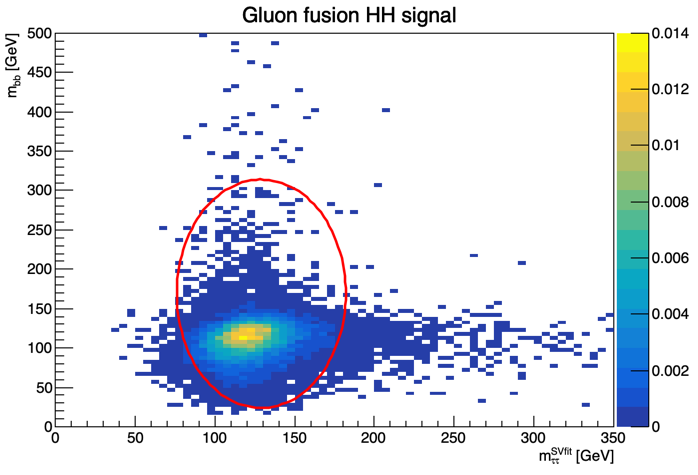
\includegraphics[width=0.45\textwidth]{Images/inclusive_2018_2b_Sig}}
%	\subfloat{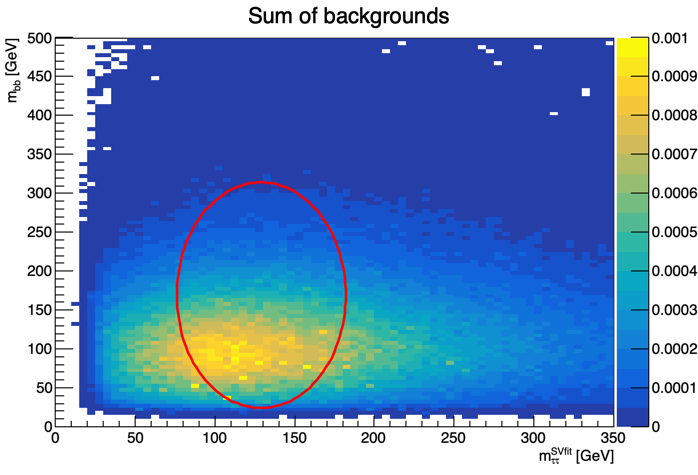
\includegraphics[width=0.45\textwidth]{Images/inclusive_2018_2b_Bkg}}
%\end{center}
%\caption{2D distributions of ($m_\text{bb}$, $m_{\tau\tau}$) for the HH SM ggF signal (left) and the sum of backgrounds (right) for events belonging to the Resolved, 2 b-tag category and the three $\tau\tau$ channels considered for 2018. The red line shows the region selected by the resolved elliptical cut.}
%\label{hh:fig:mass_cut}
%\end{figure}


\subsection{Signal extraction}
\label{hh:subsec:signal_extraction}

The eight orthogonal categories described in Section~\ref{hh:sec:event_categorization} are used for the signal extraction via a DNN developed to identify HH~$\to$~bb$\tau\tau$ events. The approach used to train the DNN \cite{hh:analysis:gilesdnn} follows the one used in the CMS di-Higgs HL-LHC projection analysis for the bb$\tau\tau$ channel \cite{hh:analysis:hh_hllhc}. The goal of the DNN is to classify events as originating either from signal (SM HH~$\to$bb$\tau\tau$ produced via ggF) or background processes by assigning to them a single prediction score. Score values closer to one indicates ``signal-like'' events, while  closer to zero, ``background-like'' events. The final DNN distributions obtained by inferring this network prediction in each category, $\tau\tau$ decay channel and year are used in the signal extraction fit.

Training is performed with the \textsc{PyTorch} \cite{hh:analysis:pytorch} algorithm interfaced with \textsc{LUMIN} \cite{hh:analysis:lumin} using all MC-driven backgrounds as background processes and SM HH~$\to$~bb$\tau\tau$ as signal. Simulated events used for training are splitted in two halves, the ones with even event number and the ones with event number. A pair of discriminators are then trained with each half of the data. At inference time, the discriminators are used to predict the classes of events in the complementary halves of the data, i.e. the one trained with even event numbers for the odd event numbers, and vice versa. This way, all MC data can be used for the training without adding a bias on the predictions that would arise if only one network was used and the same data used for training was also used for inference. To further increase the statistical robustness, each discriminator consists of 10 neural networks, each trained with a different starting random seed.

For the training, a total of 26 features (selected among over a 100) are used as input to the neural network. Both categorical (year of data taking, the $\tau\tau$ decay mode or the number of VBF jet candidates) and object features are used. From the latter, the most important features (ranked by permutation importance) are the DeepJet scores of the b jets, the invariant masses of the bb, $\tau\tau$ and HH systems and kinematic variables of the reconstructed particles.



%%%%%%%%%%%%%%%%%%%%%%%%%%% MULTI-CLASS %%%%%%%%%%%%%%%%%%%%%%%%%%%%%%%%%

\subfile{multiclass}

%%%%%%%%%%%%%%%%%%%%%%%%%%%%%%%%%%%%%%%%%%%%%%%%%%%%%%%%%%%%%%%%%%%%%%%%%

\section{Background estimation}
\label{hh:sec:background}


%%%%%%%%%%%%%%%%%%%%%%%%%%%%%% QCD %%%%%%%%%%%%%%%%%%%%%%%%%%%%%%%%%%%%%%

\subfile{qcd}

%%%%%%%%%%%%%%%%%%%%%%%%%%%%%%%%%%%%%%%%%%%%%%%%%%%%%%%%%%%%%%%%%%%%%%%%%

\subsection{Z/$\gamma^*$~+~jets}
\label{hh:subsec:dy}

The contribution of Z/$\gamma^*\to ll$ associated with jets is estimated from Monte-Carlo simulations. Samples can be produced with \textsc{MadGraph5\_aMC@NLO} at LO or NLO precisions. Sample generation with LO precision can be done in an inclusive way, with up to four jets produced at matrix element, or in different samples with different number of jets at matrix element (from one to four) or requiring two b jets. The combination of both inclusive and exclusive samples lead to large statistics for this process. However, LO modelling of the jets is not really good. NLO modelling leads to better results, although samples are only generated with up to two jets and no samples with two b jets are generated. Therefore, the lack of statistics makes NLO samples not useful. The final solution is use the samples with LO precision but improving the modelling by correcting the simulation with a data-driven method. The correction factors used in the MC samples are derived from several $Z\to\mu\mu$ sideband regions.

For the scale factor computation, data and simulated events are required to pass a selection similar to the one applied in the analysis. At trigger level, events are selected by the single-muon trigger, with $p_T$ thresholds of 22~GeV in 2016 and 24~GeV in 2017 and 2018. At offline level, events should have two muons with $p_T > 20~$GeV and $|\eta|<2.4$ and one muon should match the muon used for triggering. A vertex constraint of $d_{xy} < 0.045~$mm and $d_z < 0.2~$mm is applied to both muons, and they should satisfy the tight muon identification and tight isolation working points. Each of the two selected muons should be separated from the other by $\Delta R>0.1$, have opposite charge and an invariant mass of $m_{\mu\mu}>50~$GeV. The third lepton veto and the jet section are the same as for the analysis final states.

To reduce the QCD and t$\bar{\text{t}}$ contributions in the sideband region, a cut on the missing transverse energy is applied by requiring $E_T^{\text{miss}} < 45~$GeV.

Scale factors are estimated using 18 control regions. First, events are split in 3 regions based on the number of jets that pass the medium DeepJet b-tag working point: 0, 1 or 2. The latter is the one with the largest contribution in the phase-space of interest, since it has exactly the same final state as the signal. Then, each control region is divided in six control regions based on the $p_T$ of the reconstructed Z candidate. The six control regions are named as \textit{Very Low $p_T$}, \textit{Low $p_T$}, \textit{Medium 1 $p_T$}, \textit{Medium 2 $p_T$}, \textit{High $p_T$} and \textit{Very High $p_T$}. The $p_T$ range of each control region is shown in Table~\ref{hh:tab:dy_sf}.

\begin{table}[h!]
\begin{center}
\begin{tabular}{c | c | c | c}
$p_T$ region & $p_T$ range - 2016 & $p_T$ range - 2017 & $p_T$
range - 2018 \\\hline
Very Low $p_T$  & $0<p_T\leq 10$    & $0<p_T\leq 10$    & $0<p_T\leq 10$     \\
Low $p_T$       & $10<p_T\leq 50$   & $10<p_T\leq 30$   & $10<p_T\leq 30$    \\
Medium 1 $p_T$  & $50<p_T\leq 80$   & $30<p_T\leq 50$   & $30<p_T\leq 50$    \\
Medium 2 $p_T$  & $80<p_T\leq 110$  & $50<p_T\leq 100$  & $50<p_T\leq 100$    \\
High $p_T$      & $110<p_T\leq 190$ & $100<p_T\leq 200$ & $100<p_T\leq 200$  \\
Very High $p_T$ & $p_T> 190$        & $p_T> 200$        & $p_T> 200$       
\end{tabular}
\caption{Definition of the Z $p_T$ regions for the Z/$\gamma^*\to ll$~+~jets scale factor computation.}
\label{hh:tab:dy_sf}
\end{center}
\end{table}

In each of the 18 regions, LO Z/$\gamma^*\to ll$ MC samples are subdivided in another 18 contributions, based on the number of b-partons at Matrix Element level (0, 1, 2) and the $p_T$ of the Z boson at generator level (same $p_T$ ranges as for the sideband regions). The data distribution of the invariant mass of the muon pair is fitted simultaneously in all categories, leaving the normalization of the 18$\times$18 DY contributions floating. %The scale factors obtained are shown in Fig.~\ref{hh:fig:dy_sf}. Fig.~\ref{hh:fig:dy_sf_datamc} shows, as an example, how the distribution of $m_{\mu\mu}$ improves after applying the computed scale factors.


%\begin{figure}[h!]
%\begin{center}
%\subfloat[2016]{\includegraphics[width=0.45\textwidth]{Images/SFs_2016}}
%\subfloat[2017]{\includegraphics[width=0.45\textwidth]{Images/SFs_2017}}\\
%\subfloat[2018]{\includegraphics[width=0.45\textwidth]{Images/SFs_2018}}
%\end{center}
%\caption{Scale factors, obtained from the simultaneous fit on $m_{\mu\mu}$ in 18 control regions for the 2016, 2017, and 2018 analyses.}
%\label{hh:fig:dy_sf}
%\end{figure}
%
%\begin{figure}[h!]
%\begin{center}
%\subfloat{\includegraphics[width=0.45\textwidth]{Images/m_tt_vis_2btag_2018_noSF}}
%\subfloat{\includegraphics[width=0.45\textwidth]{Images/m_tt_vis_2btag_2018}}
%\end{center}
%\caption{Distribution of $m_{\mu\mu}$ in the sideband region defined to compute the DY scale factors where the two jets pass the medium DeepJet working point. Left plot shows the distribution without applying the obtained scale factors; right plot after applying them.}
%\label{hh:fig:dy_sf_datamc}
%\end{figure}


\subsection{Top-antitop background}
\label{hh:subsec:tt}

The contribution of the t$\bar{\text{t}}$ background is obtained relying on the MC simulation. However, while the shape of the process if well modelled by the simulation, the normalization of the background shows a disagreement with respect to the data, as can be seen in Fig.~\ref{hh:fig:ttbar_disc}.

\begin{figure}[h]
\begin{center}
\subfloat[]{\includegraphics[width=0.33\textwidth]{Images/dau1_eta_baseline_SR_MuTau}}
\subfloat[]{\includegraphics[width=0.33\textwidth]{Images/dau1_eta_baseline_SR_ETau}}
\subfloat[]{\includegraphics[width=0.33\textwidth]{Images/dau1_eta_baseline_SR_TauTau}}
\end{center}
\caption{Distributions of the $\eta$ of the first lepton in 2016 for the (a) \taumu\tauh{} channel, (b) \taue\tauh{} channel, and (c) \tauh\tauh{} channel. Note that the content of each bin is scaled by the bin width. The two channels with the biggest t$\bar{\text{t}}$ contribution (\taumu\tauh{} and \taue\tauh{}) show a data/background agreement in the $\eta$ region where more t$\bar{\text{t}}$ is expected, while good agreement can be seen where poor contamination of t$\bar{\text{t}}$ is present, which points to an issue in the t$\bar{\text{t}}$ normalization.}
\label{hh:fig:ttbar_disc}
\end{figure}

In order to solve this normalization problem, a specific t$\bar{\text{t}}$ control region has been defined and fitted to extract an scale factor to be applied to the t$\bar{\text{t}}$ background yield. This control region had to be as close as possible to the signal region but orthogonal to it, being as much enriched and pure on t$\bar{\text{t}}$ events as possible. The control region was finally defined by applying the same selections shown in Section~\ref{hh:sec:event_categorization} for the Resolved, 2 b-tag category except for the mass cut, which will be the inverse of the mass cut used in that category:
\begin{equation}
\frac{(m_{\tau\tau} - 129~\text{GeV})^2}{(53~\text{GeV})^2} + \frac{(m_\text{bb} - 169~\text{GeV})^2}{(145~\text{GeV})^2} > 1.
\end{equation}

A fit is performed in this region by including only as nuisance parameters (see Section~\ref{hh:subsec:nuisances}) this t$\bar{\text{t}}$ scale factor (that applies only to t$\bar{\text{t}}$ background) and the statistical uncertainties in each of the three years. To reduce these statistical uncertainties, the three channels are considered altogether. The results for these scale factors are found in Table~\ref{hh:tab:ttsf}.

\begin{table}[h!]
\begin{center}
\begin{tabular}{c | c | c}
2016 & 2017 & 2018 \\
\hline
$0.908 \pm 0.006$ &  $0.988 \pm 0.006$ & $0.966 \pm 0.009$
\end{tabular}
\end{center}
\caption{Results of the t$\bar{\text{t}}$ control region fits for the three years. The values of the t$\bar{\text{t}}$ scale factors and their uncertainties are reported.}
\label{hh:tab:ttsf}
\end{table}


\subfile{corrections}

%\bibliographystyle{plain}
%\bibliography{../biblio.bib}


\end{document}

